\section{Experimentacion}
El objetivo del trabajo era encontrar el \textit{mejor} arquero usando técnicas de métodos
numéricos. Qué dice qué arquero es mejor que otro es difícil de decidir cuando existen arqueros que
atajan tiros distintos pero en total la misma cantidad. En esta sección trataremos de decidir
utilizando los siguientes criterios:
\begin{compactitem}
  \item Diferencia en posición final: este criterio mide la distancia final entre la pelota y
    nuestro arquero. Si es menor a 7 entonces nuestro arquero la atajó. Además, nos sirve para ir
    analizando en el tiempo cómo es el comportamiento de nuestro arquero. \\
    Los archivos de tests correspondientes son los que contienen al substring ".movsgol".
  \item Diferencia en coordenada \texttt{y} a lo largo del tiempo: en este caso iremos viendo sólo la
    información del eje \texttt{y} para cada momento de tiempo y comparándola en el caso de la pelota
    y nuestro arquero. Nos sirve para ver cómo es el movimiento de nuestro arquero según se va
    moviendo la pelota. Una estrategia \texttt{ingenua} que no consideramos en nuestro trabajo sería
    ir acercando el arquero a cada coordenada \texttt{y} de la pelota a lo largo del tiempo, sin
    considerar que pueda cambiar bruscamente y nos alejemos demasiado del destino final.
    \\
    Los archivos de tests correspondientes son los que contienen al substring ".movstodos".
  \item Error en estimación: compara la posición de gol de la pelota contra la estimación de
    nuestros métodos. Es decir, en cada momento qué tan errada está la estimación de por dónde va a
    entrar la pelota. Sirve para ver cómo va cambiando la estimación con más información o mientras
    más se acerca al arco.
    \\
    Los archivos de tests correspondientes son los que contienen al substring ".movsestimacion".
  \end{compactitem}


\section{Resultados}

\subsection{Experimentacion con Lineales}
\begin{figure}[H]
\includegraphics[width=\textwidth]{img/lineal6_125.movsestimacion.TODOS.elegidos.ps}
     \caption{bla}
\end{figure}

\subsection{Experimentacion con Curvas}

\subsection{Experimentacion con Jugadores}

\subsection{Experimentacion con Exoticos}